\section{Theory}

%% Part1 - solar cells -> materials
Most solar cells are made from a crystalline, meaning the structure of atoms is ordered, or periodic. Generally the crystals will contain imperfections and impurities. Some solar cell materials however, is not crystalline, but are missing periodicity. These solar cells are made from amorphous materials.

\subsection{Bandgap}

A free electron in vacuum is able to have any energy. An electron in a crystal is bound by an energy gap divided by energy positions the electrons can't possess. Every available energy state can only room two electrons according to the Pauli principle. For a crystal, the energy bands can be viewed as an overlap in between single electron energy states. This can be viewed as the crystals 'electron'-shell.

\begin{figure}[H]
 \centering
 	% Tegning
 	\begin{tikzpicture}[scale=0.5]
     	\draw[very thick,->] (1,6) -- node[below] {x}  (25,6); % X akse
    	\draw[very thick,->] (1,6) -- node[left] {\begin{sideways}Energy\end{sideways}} (1,18); % Y akse
    
    \begin{scope} % Valens og ledningsb�nd
		    \draw[thick,fill=black!10] (2,7) rectangle node {Valence band} ++(22,4);
        \draw[thick,fill=black!10] (2,13) rectangle node {Conduction band} ++(22,4);
        \draw[thick,<->] (13,13) -- node[right] {Band gap} (13,11); % Pil
    \end{scope}
    \end{tikzpicture}    \caption{Energy bands}
    \label{fig:energiband}
\end{figure}

The upper band is called conduction band. The band right below it, is called the valence band. This band gap is very important in relations with solar cells, and is often given in the units of electron volts (eV).

For electrons to move out of the crystal, they have to be in the conduction band. For electrons to get to the conduction band, they need to have enough energy to move from the valence band. This can happen if the electron has enough thermal energy, or receive energy from the outside, like light. This gives the material increased conductivity. In addition to this, there will be a free state in the valence band, which results in a less probability of collisions among the remaining electron, which lead to a higher mean kinetic energy of the electrons in the valence band. This also contribute to a better conductivity for the material. 

For light to excite an electron from the valence band to the conduction band, it needs to have equal, or more energy than the band gap. Energy of light in electron volts is given by:

\begin{equation}
E=h\nu =\frac{hc}{\lambda}
\label{eq:light_energy}
\end{equation}

where $E$ is energy in electron volts, $h$ is Planks constant, $\nu$ is frequency, and $c$ is the speed of light.

Materials is often divided into three categories; Isolators, semiconductors, and conductors. Isolators have none, or few electrons in the conduction band, which gives them poor conductivity. Conductors often have filled conduction bands in room temperature, which provide good conductivity. Even with 0K, conductors have a partially filled conduction band. Semiconductors on the other hand, does not have any electrons in the conduction band at 0K. Semiconductors have lower conductivity than conductors, but better than isolators. The bandgap for semiconductors lay in between that of the conductors and isolators. At room temperature semiconductors have a partially filled conduction band.

\begin{figure}[H]
 \centering
 % Tegning
 

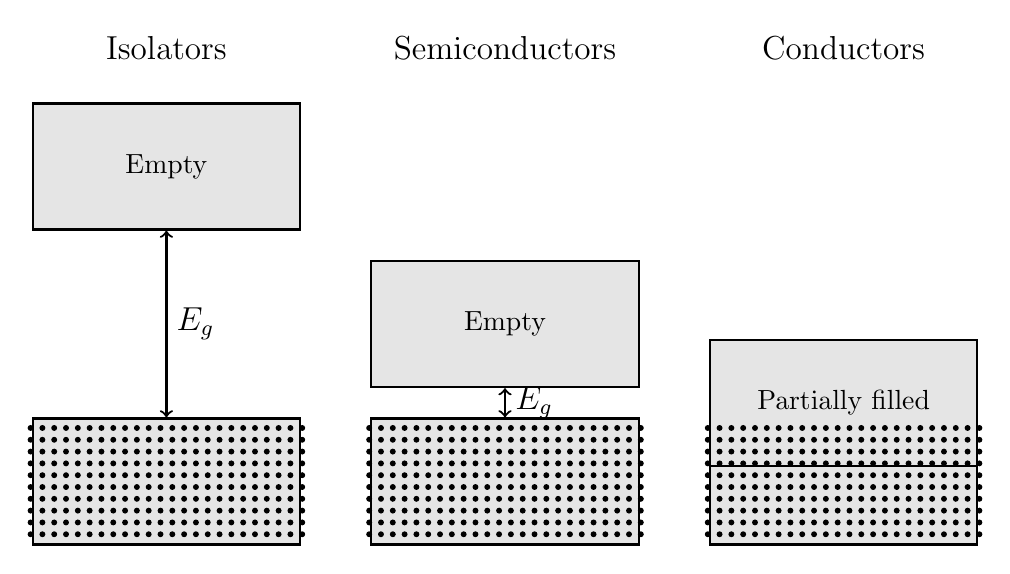
\begin{tikzpicture}
 	% Styles til elementer (kan ogs� v�re generelle utenfor tikzpicture)
	\tikzstyle{ledningsband} 	=	[rectangle, draw, thick, fill=black!10, text width=9em, text centered, minimum height=1.6cm]
	\tikzstyle{valensband}		= [rectangle, draw, thick, fill=black!10, text width=9em, text centered, minimum height=1.6cm]


	% Boksene i bunnen
	\node[valensband]	(valens_isolator)																										{};
	\node[valensband]	(valens_halvleder)	[right of=valens_isolator,  node distance=4.3cm]	{};
	\node[valensband]	(valens_metall)			[right of=valens_halvleder, node distance=4.3cm]	{};	
	
	% Boksene i toppen
	\node[ledningsband]	(lednings_isolator)		[above of=valens_isolator, 	node distance=4cm]	{Empty};
	\node[ledningsband]	(lednings_halvleder)	[above of=valens_halvleder, node distance=2cm]	{Empty};
	\node[ledningsband]	(lednings_metall)			[above of=valens_metall, 		node distance=1cm]	{Partially filled};
	
	% Piler
	\draw[thick,<->] (valens_isolator)  -- node[right] {\large $E_g$} (lednings_isolator);
	\draw[thick,<->] (valens_halvleder) -- node[right] {\large $E_g$} (lednings_halvleder);
	
	% Tekst p� toppen
	\node (isolator_tekst)  [above of=lednings_isolator,node distance=1.5cm]	{\large Isolators};
	\node (halvleder_tekst) [right of=isolator_tekst, 	node distance=4.3cm] 		{\large Semiconductors};
	\node (metaller_tekst)  [right of=halvleder_tekst, 	node distance=4.3cm] 		{\large Conductors};
	
	% Elektroner i valensb�nd
	\foreach \y in {0,0.15,...,1.4}
		\foreach \x in {0,0.15,...,3.5} {
			\draw (\x-1.725,\y-0.67) circle (0.03cm) [fill=black];	% Isolator
			\draw (\x+2.575,\y-0.67) circle (0.03cm) [fill=black];	% Halvleder
			\draw (\x+6.875,\y-0.67) circle (0.03cm) [fill=black];	% Metall
		}	
	
\end{tikzpicture}

	    \caption{Typical bandgaps at 0K} 
 \label{fig:bandgap}
\end{figure}
\vspace{10mm}

Typical bandgap for semiconductor silicon is E$_g$=1.1~eV, compared with 5~eV for diamond, which is an isolator \cite[Chapter 3]{streetman}.

Holes is a description of missing electrons in the valence band. A hole will appear when an electron is excited from the valence band into the conduction band. With a small bandgap, and high temperatures, there will be a considerably larger amount of electrons in the conduction band, compared to low temperatures, and a large bandgap. This is described by low of mass action

\begin{equation}
np=N_cN_ve^{-\frac{E_g}{kT}}
\label{eq:massevirkningsloven}
\end{equation}

where $n$ is number of electrons, $p$ is number of holes, $N_c$ and $N_v$ is constants for a given material, $E_g$ is the bandgap, $k$ is Boltzmanns constant, and $T$ is temperature in Kelvin. For an intrinsic semiconductor, meaning a semiconductor without any doping atoms, like a pure silicon crystal, the law of mass action can be written as

\begin{equation}
np=n_i^2
\label{eq:massevirkningsloven_intrinsikk}
\end{equation}

where

\begin{equation}
n_i=\sqrt{N_c N_v}e^{-\frac{E_g}{2kT}}
\label{eq:intrinsikk}
\end{equation}


\subsection{Doping}

By adding certain atoms of a different type than those constituting the semiconductor itself, it is possible in increase the concentration of electrons in the conduction band without a concomitant increase on the number of holes in the valence band. This is called donor-doping. An example of donor doping is added phosphorous into a silicon crystal. This will result in more electrons in the conduction band, due to phosphor having one more valence electron than silicon. The doping is usually so small that the band structure won't be affected. By adding phosphorous this way, one has increased electrons, $n$, without increasing holes, $p$. This is called donor doping. If you instead of phosphor, add boron, the material will be acceptor doped. This is due to boron having one less electron in the valence band than silicon, and would result in an extra hole in the valence band of the crystal. Usually the number of dopants in silicon are substantially larger than the intrinsic concentration, $n_i$, so that

\begin{equation}
n \approx N_d
\label{eq:donordoping}
\end{equation}

for donor doping, and

\begin{equation}
n \approx N_a
\label{eq:akseptordoping}
\end{equation}

for acceptor doping where $N_d$ is donor concentration, and $N_a$ is acceptor concentration.

A doped semiconductor is generally called extrinsic \cite{streetman}. If a semiconductor is doped with a number of donor atoms, it is called n-doped or n-type, due to there being more electrons than holes. For acceptor doping it is called p-doped, or p-type semiconductor. The dominating charge carrier in the semiconductor are called majority carriers. The other charge carrier, i.e. holes in the n-type semiconductor are called minority carriers.

\subsection{Transport and recombination processes}

There are two mechanisms that contribute to transport of electrons and holes in semiconductors: drift, and diffusion. Drift is a transport of a charge carrer due to an electric field. For transport of a hole in one dimension, the current $I_p$ is equal to the amount of holes $N_p$ times the charge $q$ crossing a cross-sectional area.

\begin{equation}
I_p = N_p q
\label{eq:drift}
\end{equation}

In vacuum, an electric field would accelerate the electrons, and the velocity would increase indefinitely. In solids, however, interactions of collisions with other species in the solid leads to a resistance towards the drift of the charged particles, and after an initial acceleration the velocity becomes constant in a constant electric field. This average drive velocity, denoted $v_p$ for holes, is related to the electric field $E$ through the hole mobility $�_p$

\begin{equation}
v_p = �_p E
\label{eq:electronspeed}
\end{equation}

If all the electrons is moving in the same direction, the current per area is given by

\begin{equation}
J_p = \frac{I_p}{A} = \frac{N_p q}{A} = pAv_p \frac{q}{A} = pv_p q = pq�_p E
\label{eq:hulltetthet}
\end{equation}

combined with a similar expression for electrons

\begin{equation}
J = J_p + J_n = (nq�_n + pq�_p)E = \sigma E
\label{eq:stromtetthet}
\end{equation}

where $�_n$ is the mobility for electrons,$\signa$ is the semiconductors conductivity, and $J_n$ is the current density due to the concerted movement of electrons. It is also usual to define the resistivity of the semiconductor as the inverse of its conductivity. The current is then obtained by

\begin{equation}
I = JA = A\sigma E = \left( \frac{A\sigma}{L}\right)V
\label{eq:current}
\end{equation}

which is recognized as Ohm's law.


Diffusion is a transport process caused by the random motion of the diffusing particles in the medium in which they diffuse. The net transport of particles is in the opposite direction of the concentration gradient. For holes we have

\begin{equation}
N_p=-D_p\frac{dp}{dx}
\label{eq:diffusion}
\end{equation}

where the proportionality constant $D_p$ is the diffusion coefficient (m$^2$/s) for holes.

The movement of charged particles are frequently determined by the simultaneous presence of electric fields and concentration gradients. Both of the relevant transport parameters, mobilities and diffusion coefficients, will in general depend on temperature. The relation between diffusion coefficient and mobility is

\begin{equation}
\frac{D_p}{\my_p}=\frac{kT}{q}
\label{eq:transport_relation}
\end{equation}

for holes, and a corresponding one exist for electrons.

\subsection{Excitation and recombination}

Electrons can move from one band to another directly, or indirectly. In indirect generation and recombination the electrons employ the so-called gap-states. Such conditions will always exist in semiconductors and are related to impurities, defects in the crystal structure, boundary surfaces (grain boundaries) and surfaces. Gap-states are in between the valence band and the conduction band, which is not allowed states in a perfect crystal.


\begin{figure}[H]
\centering
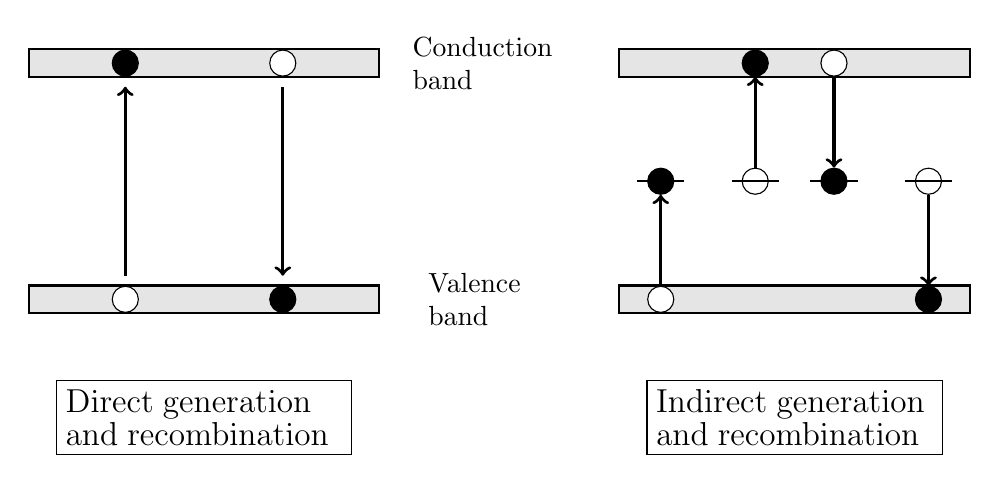
\begin{tikzpicture}

% Styles til elementer
\tikzstyle{band} 	=	[rectangle, draw, thick, text width=12em, fill=black!10, text centered, minimum height=1em]
\tikzstyle{e} 	=	[circle, draw, fill=black] % radius=0.2cm
\tikzstyle{h} 	=	[circle, draw, fill=white] % radius=0.2cm

	% Direkte
	\node[band]	(direkte_valens)																									{};
	\node[band]	(direkte_lednings)	[above of=direkte_valens, node distance=3cm]	{};
	\node[e] (elektron1) [right of=direkte_valens] {}; % Elektron
	\node[h] (hull1) [left of=direkte_valens] {}; % Hull
	\node[e] (elektron2) [left of=direkte_lednings] {}; % Elektron
	\node[h] (hull2) [right of=direkte_lednings] {}; % Hull
	\draw[very thick,->] (-1,0.3) -- (-1,2.7) {} ; % Pil opp
	\draw[very thick,<-] (1,0.3) -- (1,2.7) {} ; % Pil ned
	\node (direkte_tekst) [rectangle, draw, text width=10em, below of=direkte_valens,node distance=1.5cm]	{\large Direct generation and recombination};
	
	\node (lednings_tekst) [right of=direkte_lednings, node distance=3cm, text width=2em] {Conduction band};
	\node (valens_tekst) [right of=direkte_valens, node distance=3.2cm, text width=2em] {Valence band};
	
	% Indirekte
	\node[band]	(indirekte_valens)		[right of=direkte_valens,  node distance=7.5cm]	{};
	\node[band]	(indirekte_lednings)	[above of=indirekte_valens, node distance=3cm]	{};
	
	\node[h] (h3) [left of=indirekte_valens, node distance=1.7cm] {}; % Hull
	\node[e] (e3) [above of=h3, node distance=1.5cm] {}; % Elektron
	\draw[very thick,->] (h3) -- (e3) {}; %Pil
	\draw[thick,-] (5.5,1.5) -- (6.1,1.5) {}; % Linje gjennom
	
	\node[e] (e4) [left of=indirekte_lednings, node distance=0.5cm] {}; % Elektron
	\node[h] (h4) [below of=e4, node distance=1.5cm] {}; % Hull	
	\draw[very thick,->] (h4) -- (e4) {}; % Pil
	\draw[thick,-] (6.7,1.5) -- (7.3,1.5) {}; % Linje gjennom
	
	\node[h] (h5) [right of=indirekte_lednings, node distance=0.5cm] {}; % Hull
	\node[e] (e5) [below of=h5, node distance=1.5cm] {}; % Elektron
	\draw[very thick,->] (h5) -- (e5) {}; % Pil
	\draw[thick,-] (7.7,1.5) -- (8.3,1.5) {}; % Linje gjennom
	
	\node[e] (e6) [right of=indirekte_valens, node distance=1.7cm] {}; % Elektron
	\node[h] (h6) [above of=e6, node distance=1.5cm] {}; % Hull	
	\draw[very thick,->] (h6) -- (e6) {}; %Pil
	\draw[thick,-] (8.9,1.5) -- (9.5,1.5) {}; % Linje gjennom
	
	\node (indirekte_tekst) [rectangle, draw, text width=10em, below of=indirekte_valens,node distance=1.5cm]	{\large Indirect generation and recombination};
	
\end{tikzpicture}	

\caption{Generation and recombination}%
\label{fig:indirect}%
\end{figure}

In semiconductors with direct bandgap, like GaAs, both processes will occur. In semiconductors with with indirect bandgap, like silicon, a direct process cannot happend without contributions from lattice vibrations (phonons), something which makes the process less probable. In semiconductors with indirect bandgap, indirect generation, and recombination will dominate. %%%%%%%% check english litterature - streetman etc.

% Indirekte b�ndbap figur
\begin{figure}[H]
\centering
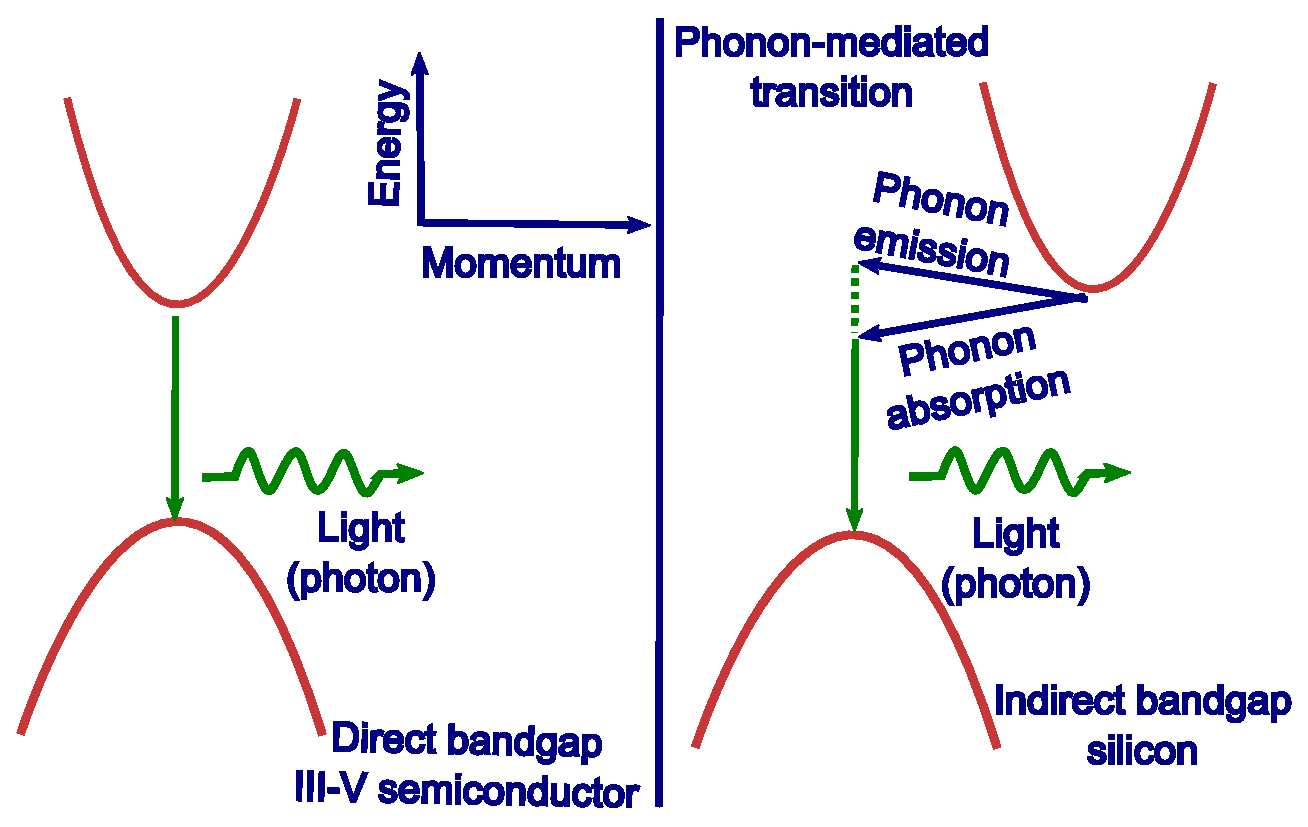
\includegraphics[width=\columnwidth]{bandgap}%
\caption{Direct and indirect recombination (figure from \cite{aps})}%
\label{fig:indirect_direct}%
\end{figure} % Solar cells
\subsection{Material science}

A commonly used semiconductor for solar cells, is silicon. The supply of silicon is practically endless. 60\% of the Earth's crust is sand, for the major part SiO$_2$. Metallurgical grade silicon (MG-Si) is produced in large amounts to make special steel alloys. Its purity is only 99\% - insufficient for electronic applications \cite{solar_cells}. 

The semiconductor industry purifies this metallurgical-grade silicon until the purity is better than 99.99999~\%. This corresponds to less than 0.1~ppma (part per million atomic), meaning that the total number of foreign atoms must be less than 5$\cdot$10$^{15}$~cm$^{-3}$, due to silicon crystalline atoms density of 5$\cdot$10$^{22}$~cm$^{-3}$ \cite{solar_cells}.

Semiconductor-grade silicon is about ten times more pure than solar-grade silicon. That means that solar-grade silicon can contain up to 1~ppma impurities and still permit reasonably efficient cells. This allows for a lower cost purification process.

\subsubsection{Czochralski method}

The most common crystallization method used for both microelectronoic and photovoltaic industries is the Czochralski method (CZ) ,  shown in figure \ref{fig:czochralski_process} \cite{solar_cells}.

\begin{figure}[H]
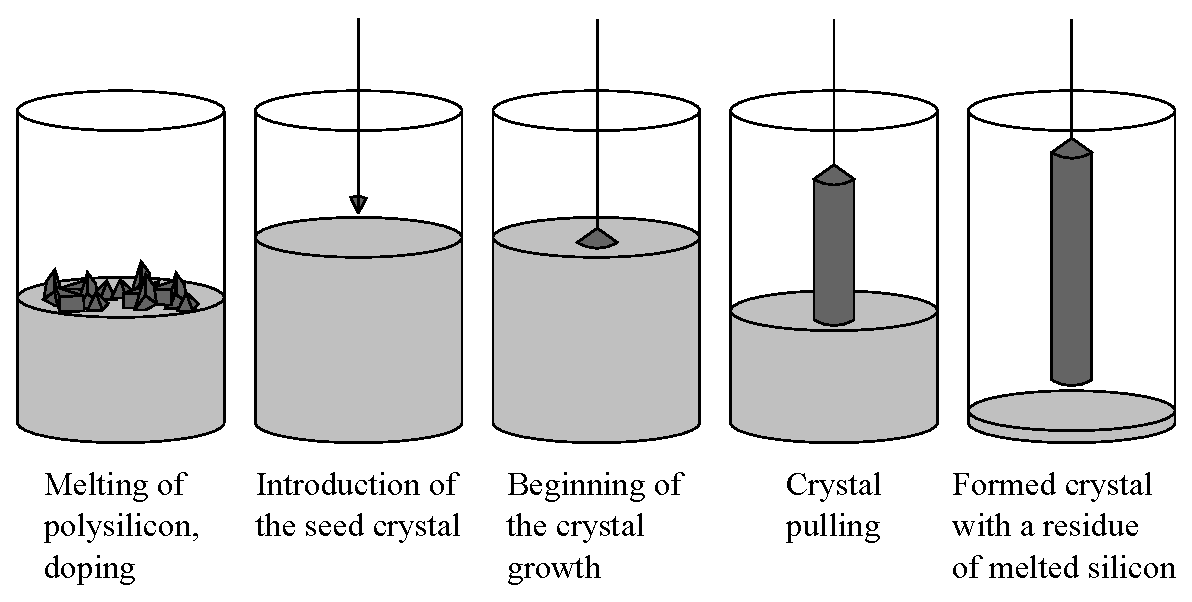
\includegraphics[width=\columnwidth]{Czochralski_Process}%
\caption{Czochralski process}%
\label{fig:czochralski_process}%
\end{figure}

In the CZ crystal growth, silicon chunks are first melted at 1414$^\circ$C in a graphite crucible lined with high purity quartz (SiO$_2$). This known as a feedstock. A small polysilicon crystal is used as a seed to start the crystallization process. The seed is carefully put in contact with the melt and then pulled out very slowly. The temperature is controlled, so that the silicon solidifies at the interface between the seed and the melt and the atoms arrange themselves according to the crystallographic structure of the seed. The crystal grows both vertically and laterally, aided by a rotation movement, yielding a cylindrical ingot of single-crystal silicon. 

The growth rate in the CZ method is about 5~cm/h and the cylindrical ingots are typically 1~m long, 20~cm in diameter and 75~kg in weight \cite{solar_cells}. A disadvantage of the CZ method is that the interaction between the molten silicon and the crucible introduces some contamintants, in particular carbon and oxygen. 

\subsubsection{Float-zone process}

The highest quality silicon crystals are obtained by using the float-zone process. In this method, the starting polysilicon is first given the shape of a cylindrical bar. The bar is then locally melted by a coil using radio frequency induction. By moving the coil, and hence the molten zone, along the bar starting from the seed end, the silicon adopts the crystalline structure. The molten zone is self-supporting and is never in contact with a foreign material, thus avoiding contamination problems. The typical growth rate is 15-30~cm/h, and the typical ingot is 15~cm in diameter and 1~m in length.

\subsubsection{Siemens process}

In the Siemens reactor process, trichlorosilane gas is introduced into a thermal decomposition furnace (reactor) exposing high-purity silicon rods at 1150~$^\circ$C. The trichlorosilane gas decomposes and deposits additional silicon onto the rods, enlarging them:

\begin{equation}
2 \text{HSiCl}_3 \rightarrow 2 \text{HCl} + \text{SiCl}_4
\label{eq:siemens}
\end{equation}

The silicon contained in the gas will deposit on the heated rods, which gradually grow until the desired diameter has been reached. The end product is in the form of rods or chunks of polysilicon. The technology in the Siemens reactor is widely implemented, accounting for a majority of the polysilicon production today, and produce a high purity material \cite{pv_handbook}.


\subsubsection{Multicrystalline silicon}

In order to reduce cost, and increase production rates, the multicrystalline silicon (mc-Si) production method was developed. It is possible to grow silicon ingots by simply melting the starting material, typically silicon scrap, into a crucible, and carefully controlling the cooling rate. Upon cooling, a directional solidification takes place and relatively large crystals grow in a columnar way. A crystalline seed is not used, and the nucleation of the silicon atoms commences in many places simultaneously, leading to a myriad of crystals (or grains) of arbitrary shape and crystallographic orientation. Each grain is several millimeters to centimeters across, and internally it has the same structure as single crystalline silicon. The boundaries between the different grains (grain boundaries), are the most obvious imperfection in the material, but they are not the only ones. Microdefect are also common and contamination from the crucible can happen as well, not to mention the possible impurities present in the starting silicon. This means that the mc-Si typically has lower electronic quality than the material produced by other methods, like the CZ method. Mc-Si typically contains much less oxygen then CZ-Si, due to CZ-Si is more exposed to air during the manufacturing process. The typical crystallization rate is 3.5~kg, and the growth cycle of a complete 16~kg ingot takes 46~h \cite{solar_cells}. 

\subsubsection{Wafers}

The silicon ingots have to be sliced into wafers. Before this they are shaped to meet dimensional specifications. The cylindrical CZ ingots are usually reduced to a quasi-square shape. This implies a loss of about 25~\% of the material, but is necessary if a high packing factor of the cells in the module is required. The large cast silicon parallelepipeds are sawn into smaller bricks. In the case of mc-Si ingots, the shaping is also used to discard the peripheral regions that are usually heavily contaminated by the crucible, which represents approximiately 15~\% of the ingot. In the photovoltaic industry, the wafers are cut by a multi-wire saw machines, that can cut simultaneously whole blocks, thus increasing the throughput dramatically (figure \ref{fig:wire_saw}).

\begin{figure}%
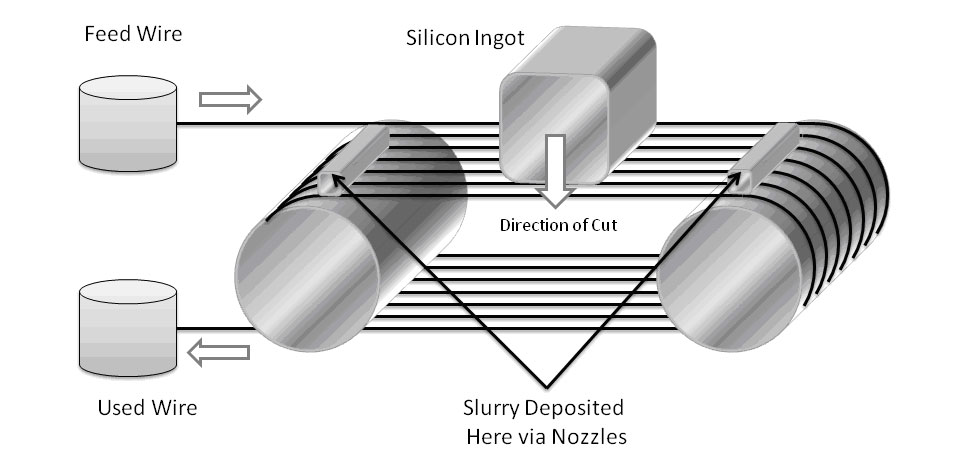
\includegraphics[width=\columnwidth]{wire_saw}%
\caption{Wafer wire saw (figure from \cite{wire_saw})}%
\label{fig:wire_saw}%
\end{figure}

An abrasive slurry helps the steel wires cut through silicon, which is a very hard material. The cutting is very slow, with eight hours being typically needed to cut through a 10x10~cm$^2$ block. Despite this advanced technique, slicing remains as one of the most costly steps of the whole silicon solar cell fabrication. Even if very thin wires are used, approximately 30~\% of the silicon is wasted as saw dust \cite{solar_cells}.


\subsubsection{Doping}

A controlled amount of boron or phosphorus is usually added to the melt (feedstock) to dope the silicon p- or n-type. Rather than the elemental boron or phosphorous, accurately measured amounts of silicon, heavily doped with those elements, are added to the melt. The typical boron concentration used for solar cell applications is 1.5$\cdot$10$^{16}$~cm$^{-3}$, which results in a resistivity of 1~\ohm cm \cite{solar_cells}.


\subsubsection{Defects}

Crystals possess imperfections. They are often referred to as crystalline defects. The presence of most of these crystalline defects is undesirable in silicon wafers. Crystalline defects may be classified into four categories according to their geometry; zero-dimensional or point defects, one-dimensional or line defects, two-dimensional or area defects, and three-dimensional or volume defects

\begin{table}[H]
\begin{tabular}{|c|c|}

\hline
\textbf{Defect type} & \textbf{Examples} \\ \hline

\multirow{4}{*}{Point or zero-dimensional defects} & Vacancy defects \\
 & Interstitial defects \\
 & Frenkel defects \\
 & Extrinsic defects \\ \hline
 
\multirow{2}{*}{Line or one-dimensional defects} & Straight dislocations (edge or screw) \\
 & Dislocation loops \\ \hline
 
\multirow{3}{*}{Area or two-dimensional defects} & Stacking faults \\
 & Twins \\
 & Grain boundaries \\ \hline

\multirow{2}{*}{Volume or three-dimentional defects} & Precipitates \\
 & Voids \\ \hline

\end{tabular}
\caption{Examples of crystalline defects from \cite{siliconfareast}}
\label{tab:crystalline_defects}
\end{table}

Vacancy defects are defects where a silicon atom is missing in the crystal structure. If an atom is located at a non-lattice location within the crystal, it is known as an interstitial defect. If the interstitial defect involves a silicon atom at an interstitial site within a silicon crystal, then it is referred to as a self-interstitial defect. Vacancies and self-interstitial defects are classified as intrinsic point defects \cite{siliconfareast}.
            
A Frenkel defect, is when an atom vacates its position in the crystal lattice to an interstitial position. Extrinsic point defects involve a foreign atom, and are more critical than intrinsic point defects. If this foreign atom replace a silicon atom in the lattice, it becomes a substitutional impurity. This include impurity atoms like the dopants B and P. Other common impurities are oxygen, carbon, and metals \cite{davies88}.


Dislocations, or crystal line defects consists of edge dislocations, screw dislocations or a combination of the two. Edge dislocation can be described as an extra plane of atoms squeezed into a part of the crystal lattice. The location with extra atoms would be under compressive stresses, while the part with correct number of atoms would be under tensile stresses. The line connecting all the atoms at the end of the extra plane is known as the dislocation line.

Screw dislocation is such that a step or ramp is formed by the displacement of atoms in a plane in the crystal. The dislocation line of a screw dislocation is in the axis of the screw.


\begin{figure}[H]
\centering
\subfigure[An edge dislocation]{
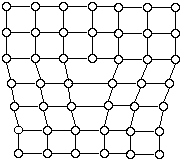
\includegraphics[width=.45\columnwidth]{edge_dislocation}
\label{fig:edge_dislocation}
}
\subfigure[A screw dislocation from \cite{siliconfareast}]{
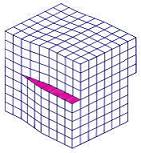
\includegraphics[width=.45\columnwidth]{screw_dislocation}
\label{fig:screw_dislocation}
}
\label{fig:dislocations}
\caption{Dislocations}
\end{figure}

Dislocation loop is a closed curve consisting of an extra plane of atoms lying entirely within the crystal. The line usually form a circular shape, since this shape results in the lowest dislocation energy \cite{siliconfareast}.

Dislocations are not wanted in silicon wafers because impurities are known as recombination centers \cite{tarasov00} and serve as sinks for metallic impurities. Gettering may also occur at dislocations, which can lead to the formation of precipitates.


Stacking faults can be considered as a disturbance in the regularity of the stacking of planes in a crystal lattice. This can occur when a plane is inserted or removed from the lattice. Stacking faults can become electrically active when decorated by impurity atoms. Such stacking faults can lead to device degradation.

A twin is a mirroring of a regular lattice formed during the growth of the silicon ingot. This is usually caused by perturbation. The twin boundary is the mirror plane of the twin formation as seen in figure (\ref{fig:twin_boundary});

\begin{figure}[H]
\centering
\subfigure[Stacking faults from \cite{stacking_faults}]{
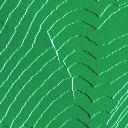
\includegraphics[width=.45\columnwidth]{stacking_fault}
\label{fig:stacking_faults}
}
\subfigure[Twin boundary]{
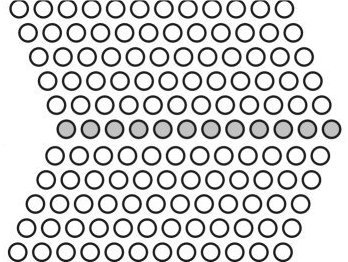
\includegraphics[width=.45\columnwidth]{twin_boundary}
\label{fig:twin_boundary}
}
\label{fig:dislocations_types}
\caption{Area defects}
\end{figure}

Grain boundaries are the boundary in between individual grains where crystal orientation is different from one another. This is common in mc-Si samples due to the production method.
     
Bulk or volume defects include voids and precipitates of extrinsic and intrinsic point defects. Impurities in a crystal which are introduced at a high temperature usually have a higher solubility than for lower temperatures. If the maximum concentration of an impurity allowed by its solubility at high temperature, the crystal become supersaturated with that impurity once it is cooled down. Under such supersaturated conditions, the crystal seeks and achieves equilibrium by precipitating the excess impurity atoms into another plane phase of different composition or structure. Precipitates are undesireable because they can act as sites for generation of dislocations. Precipitates can form in silicon from metallic impurities, oxygen and dopants like boron \cite{siliconfareast}.




%% Part 2 - Spectroscopy properties of Si


% band structure
% phonons
% Excitons
% EHD
% Different kinds of recombination in impurities/defects %% FIGURE (trap states, EHD, excitons etc.)
% Temperature dependance
\subsection{Spectroscopic properties of silicon}

When an electron hole pair is recombining, the energy is released as a photon. By measuring this photon in a photo detector it can be determined how much energy that was released during recombination. This energy tells how large the bandgap is, which in turn tells us something about the material. By shining light with high enough energy and intensity on to a sample, the light will excite electrons into all available states. When these states recombine, the emitted light can be detected by a camera as a spectra of different wavelengths. The fundamental energy gap between the valence and conduction bads in silicon is indirect, decreasing monotonically from 1.170~eV at 0~K to ~\1.125~eV at room temperature \cite{davies88}. The main phonon contribution (TO phonons) result in energies \~1.1~eV for the emitted photons. If there are impurities or defects in the silicon crystal, they can in turn emit light at different photon energies.



% band structure
% phonons
% Excitons
% EHD
% Different kinds of recombination in impurities/defects %% FIGURE (trap states, EHD, excitons etc.)
% Temperature dependance

% Spectroscopy (header)
% as method
% how to cool down a sample / cryo
% What is a cryostat
% different types of cooling, He, N etc.

% Excitation of sample
% different wavelengths, give list of inntrengingsdybde for forskjellige b�lgelengder
% spot size ++

\begin{figure}[H]
\centering
%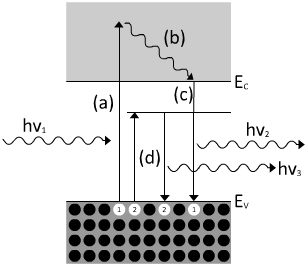
\includegraphics[width=10cm,bb=0 0 306 265]{luminisence.png}%
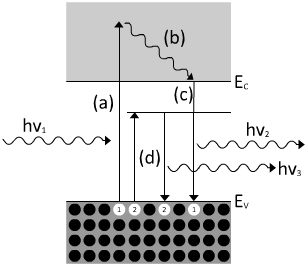
\includegraphics[width=10cm]{luminisence}%
\caption{Excitation and recombination \cite{streetman}}%
\label{fig:luminescence}% 
\end{figure}

Figure \ref{fig:luminescence} show incoming light with high intensity in a direct band gap material. In $a$, an electron is excited to a high energy state, which falls down to a lower energy state in $b$, after a very short time. When this electron recombines in $c$, it emits a photon with energy equal to $E_c$. Another electron is excited in $d$, which reach a so-called trap state, which can occur from impurities in the crystal, or defects. This trap state have a lower energy than the band gap, and when this electron hole pair recombines, and lower energy is emitted. By looking at the light from such trap states, certain known spectra related to different impurities and defects can be recognized.

For an indirect band gap material like silicon, there are other energy levels than the band gap to consider:

\subsubsection{Phonons}

A phonon is an elastic wave in a material such as a silicon crystal. It can be described as lattice vibrations, where the phonon propagate with wave vector $\vec{k}$. There is longitudinal (LA), transverse acoustical (TA), longitudinal (LO), and transverse optical (TO) modes. 

\begin{figure}[H]
\centering
\subfigure[Optical mode]{

\includegraphics[width=.45\columnwidth]{transvere_optical_mode}
\label{fig:transvere_optical_mode}
}
\subfigure[Acoustical mode]{

\includegraphics[width=.45\columnwidth]{transvere_acoustical_mode}
\label{fig:transvere_acoustical_mode}
}
\label{fig:transverse_phonon_modes}
\caption{Transverse phonon modes}
\end{figure}

The atoms in the crystal vibrate against each other, but their center of mass is fixed. If the two atoms carry opposite charges, we may excite a motion of transversal optical with the electric field of a light wave, so that the branch is called the optical branch. If the atoms move together, as in long wavelength acoustical vibrations, whence the term acoustical branch.

Since an electron-hole pair in silicon needs a phonon to recombine, the energy of which the emitted photon has, is highly dependant on the phonon energy involved, as well as the band gap. At absolute zero temperature, a crystal lattice lies in its ground state, and contains no phonons. A lattice at a non-zero temperature  has an energy that is not constant, but fluctuates randomly about some mean value. These energy fluctuations are caused by random lattice vibrations, which can be viewed as a gas of phonons. Due to a vast amount of phonons at room temperature, the energy released by recombination varies due to larger fluctuations. In silicon, the optical modes are found right above 48 meV, transverse acoustic (TA) modes are right below 25 meV, and LA modes are in between \cite{aksamija07}. \cite{davies88} list phonon energies in silicon as 

\begin{table}[H]
\centering
\begin{tabular}{cc}
18.4$\pm$0.2~meV & TA mode \\
56.2$\pm$1~meV & LO mode \\
58.0$\pm$1~meV & TO mode \\
\end{tabular}
\caption{Phonon modes in silicon from \cite{davies88}}
\label{tab:phonon_energies}
\end{table}


\subsubsection{Excitons}

An exciton is a quasi particle describing an electron bound to a hole. Electrons can be bound together by their attractive coulomb interaction, just as an electron is bound to a proton form a neutral hydrogen atom. An exciton can move through the crystal and transport energy, however it does not transport charge because it is electrically neutral.

\begin{figure}[H]
\centering
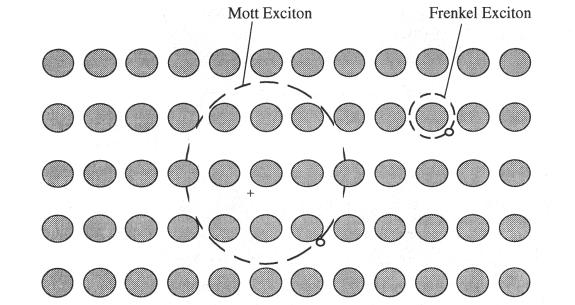
\includegraphics[width=\columnwidth]{exciton}%
\caption[Excitons]{The Mott-Wannier exciton usually free to move together through the crystal, and is weakly bound, with an average electron-hole distance large in comparison with the lattice constant. An ideal Frenkel exciton will travel as a wave throughout the crystal, but the electron is always close to the hole.}%
\label{fig:excitons}%
\end{figure}

Excitons can be formed in every insulating crystal. When the band gap is indirect excitons near the direct gap may be unstable with respect to decay into a free electron and a free hole. All excitons are unstable with respect to the ultimate recombination process in which the electron drops into the hole. Excitons can also form complexes, such as a biexciton from two excitons \cite{kittel}. In the formation of excitons, the energy is lowered with respect to the binding energy of the exciton. For silicon, the binding energy is 14.7~meV \cite{kittel}. In a tightly bound exciton (Frenkel) the excitation is localized on or near a single atom. The hole is usually on the same atom as the electron although the pair may be anywhere in the crystal.

\begin{figure}[H]
\centering
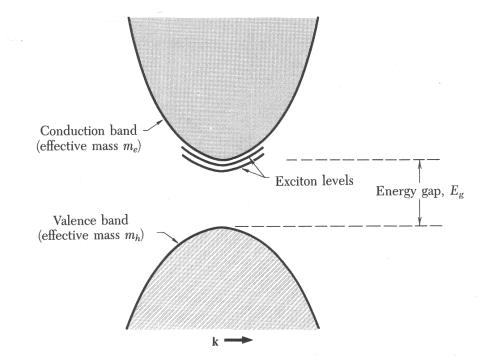
\includegraphics[width=\columnwidth]{exciton_levels}%
\caption[Excitation levels]{Exciton levels in relation to the conduction band edge for a simple band structure with both conduction and valence band edges at $\vec{k}$=0}%
\label{fig:exciton_levels}%
\end{figure}

%% B bound, P bound, energy levels ?

\subsubsection{Electron-hole drops}

A condensed phase of an electron-hole plasma forms in Ge and Si when maintained at a low temperature and irradiated by light. When an electron-hole drop (EHD) forms, the absorption of a photon produces a free electron and free hole with high efficiency. These combine rapidly to form an exciton. If the exciton concentration is sufficiently high, most of the excitons will condense into a drop. The binding energy relative to free exciton is 9.3~meV in silicon with 3.5\cdot10$^{18}$~cm$^{-3}$ $n$ or $p$ at 23K \cite{kittel}.


%% figure with multiple bandgap shortages present

\subsection{Spectroscopy}

On recombination of an electron-hole pair, it is emitted a photon. By detecting this photon it is possible to describe features about the sample. In order to generate electron-hole pairs, the sample can be excited by a laser. The laser wavelength have to be such that the energy of the light is larger than the band gap, in order to excite the sample. 

\subsubsection{Pumping wavelength}

Pumping light needs to have enough energy to fill all available states in the crystal lattice, in order to detect defects and impurities. For silicon, which has a band gap of around 1.1eV, has most impurity/defect bands below the band gap. In order to fill these states, the pumping wavelength should be below 1125nm, which corresponds to energies just over 1.1eV.

Silicon has different absorption lengths for different wavelengths. Absorption length is about 1~$�$m for 532~nm laser excitation, which means that precipitates, and defects deeper in the sample won't be detected. Like iron precipitates in \cite{gundel09}. This limitation might be overcome by an excitation laser with a longer wavelength, and consequently absorption length in silicon. For 1125nm, the absorption depth is nearly 200~$�$m \cite{laserdybde}. Compared to absorption length for 532nm, 1125nm reach 200 times deeper into the sample.


\subsubsection{Spot size}

Having a small diameter on the pumping laser allows for a high resolution of characteristics on the sample. In an iron contaminated sample, \cite{gundel09} show that at some distinct spots of a size between 1$�$m and 4$�$m, the band to band photoluminescence peak is particular low at spots with iron precipitates. 

A large electron hole droplet could overshadow characteristics from impurities in the sample. \cite{satoshi04} show that electron hole droplets become more intense for a smaller volume, with a silicon nanolayer smaller than the absorption depth of the laser. \cite{satoshi04} used a 488nm pumping laser with 1,5$�$m diameter, on silicon nanolayer thickness of 50nm and 340nm. For the 50nm layer, \cite{satoshi04} observed a large electron hole droplet, even for small pumping intensities, with the same amount of photo excited carriers per volume as for the 340nm layer. Assuming that a small volume give rise to a larger electron hole droplet, it would be a limiting factor for the spot size and pumping wavelength.

\subsubsection{Laser intensity}

With a large pumping intensity, an electron hole droplet become visible in the specter around 1.08eV in bulk silicon \cite{hammond75}. \cite{satoshi04} show that electron hole droplets occur at weak excitations (0.75mW) and even at high temperatures for a silicon nanolayer of 50nm. For thickness of 340nm, the electron hole droplet show up at pumping intensity of 3mW and above, and the intensity of the electron hole droplet grow larger than for the free exciton at 15mW. This electron hole droplet is not wanted, as it can mask characteristic photoluminescence from impurities.

With a larger pumping intensity, the impurity photoluminescence would in some cases also increase. Photoluminescence from chromium bound with a boron atom is known to increase linearly with laser power \cite{conzelmann82,conzelmann83}, and would be easier to detect at a higher pumping intensity.



\subsubsection{Temperature dependency}

At room temperature, there's a large probability that the phonon energy involved in recombination has an energy considerably different from the mean value, compared to temperatures close to 0K. This makes it difficult to separate phonon assisted recombination, from other available states, like direct recombination trap states. Trap states are important because they describe impurities by exact photon energies, which in turn makes it possible to recognize known impurities. But any recombination involving phonons will have a substantial broadening in regards to energy at room temperature.

To overcome the problem distributed phonon energies, the sample can be cooled down. When cooling down, there are less phonon states available, leading to a much narrower energy distribution of the phonons. This is desirable when looking at the photoluminescence, in order to recognize known spectra. 

Low temperatures, and high exciting laser light intensity can lead to electron-hole drops. Temperature is a substantial limiting factor for measuring silicon luminescence spectra, meaning low temperature is key to analyze silicon photoluminescence. Electron-hole drops are undesirable because they don't carry information about the material itself, and can emit light at the same wavelengths as actual material properties would. This is a limiting factor at low temperatures on the laser intensity, spot size, and wavelength.

A common way to cool down a sample, is to use liquid nitrogen. Nitrogen has a boiling temperature of 77K, so by exposing the sample to boiling nitrogen, it is cooled down. This can be done is a cryostat, which essentially is a vacuum chamber with a sample holder, where the sample holder is being cooled down. This way there will be no nitrogen contaminants on the sample itself, with only the sample holder being cooled down by nitrogen directly. It's also common to mount the sample holder on piezo elements, which can be used to move the sample in xyz directions. 

For silicon, 77K still leads to substantial broadening of emitted photon energies. In order to reach lower temperatures, a different coolant can be used. By using helium, which has a boiling temperature of 4.2K, the energy broadening is reduced to negligible values, and sharp lines from the photoluminescence can be detected.
%% To solve this -- low temperatures -- cryostat -- Helium, Nitrogen, bathind in liquid helium, compared to cryostat - cryo cryo lala

% Spectroscopy (header)
% as method
% how to cool down a sample / cryo
% What is a cryostat
% different types of cooling, He, N etc.

% Excitation of sample
% different wavelengths, give list of inntrengingsdybde for forskjellige b�lgelengder
% spot size ++

%% Part 3 - Collection of luminescence

% Optics, numerical aperture, focal plan, leses, grating/filtering, detection path components, CCD, pixel array, resolution, spatial and spectroscopy resolution (nm and ev)
% Optics, numerical aperture, focal plan, leses, grating/filtering, detection path components, CCD, pixel array, resolution, spatial and spectroscopy resolution (nm and ev)

\subsubsection{Spectrometer}

In order to analyze different wavelengths, they need to be separated, and detected individually. This is done in a spectrometer. By shining light on a diffraction grating, the light is reflected at different angles by

\begin{equation}
d\sin(\theta _m)=m\lambda
\label{eq:grating_equation}
\end{equation}

where $d$ is the distance between the grating lines, $\theta _m$ is the outgoing angel of the light, $m$ is an integer denoting the diffraction order, and $\lambda$ is the wavelength. For large wavelength resolution, the angle of the reflected light will be large as well. So, in order to measure a large specter of wavelengths, several measurements with different center wavelengths is needed. This is due to physical limitations regarding the photo detector. There is a limit to how small a single pixel can be, and how long the array of pixels you can fit in the system. Each pixel translate to a separate wavelength, which measure the intensity of that wavelength only, which result in a full spectra of wavelengths and intensities. 

\subsubsection{Optics}

For silicon luminescence, the interesting wavelengths is from 900 to 1600nm, which corresponds to 1.38~eV and 0.77~eV (see table \ref{energy_bands}). To collect this light, the optics should have minimum loss for these wavelengths.

A common way to measure photoluminescence is to send the laser excitation light through a beam splitter, which reflects 50\% of the laser light on to the sample. Then the luminescence pass through the same beamsplitter, where 50\% is trasmitted, and into the spectrometer. For micro-photoluminescence, it's desireable to hit a very small area of the sample (order of 1~$�$m). This can be achieved by using an objective. The objective focuses the excitation laser beam with a size given by the objective spesifications in the focal plane, which is the plane of focus for the objective. The length to this plane from the objective (or other optical system), is given by its numerical aperture which in turn is given by:

\begin{equation}
NA=n sin(\theta)
\label{eq:NA}
\end{equation}

where $n$ is the refractive index of the medium in which the lens is working (1.0 for air, 1.33 for pure water), and $\theta$ is the half-angle of the maximum cone of light that can enter or exit the lens.

\begin{figure}[H]
\centering
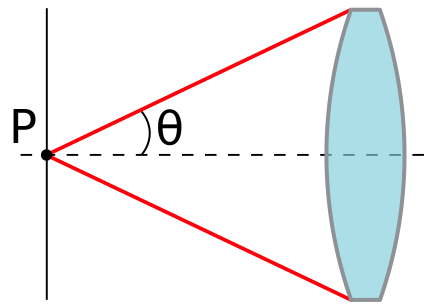
\includegraphics[width=0.5\columnwidth]{Numerical_aperture}%
\caption[Numerical aperture]{The numerical aperture with respect to a point $P$ depending on the half-angle $\theta$}%
\label{fig:NA}%
\end{figure}

where the point $P$ is the focus point. NA is important since it indicates the resolving power of a lens. The size of the details that can be resolved is proportional to $\lambda/NA$, where $\lambda$ is the wavelength of the light. A lens with a larger numerical aperture will be able to visualize finer details than a lens with a smaller numerical aperture. Lenses with larger numerical apertures also collect more light which is essential to detect luminescence of lower intensities. 

\subsubsection{Noise}

In addition to the actual photoluminescence signal, there will be noise. Noise can be from stray light in the surrounding environment hitting the camera, or it can noise from the electronics in the camera itself. Examples of noise are thermal noise, dark current, uneven amplification for different pixels in the detector, second (or more) order diffracted light from other wavelengths, background noise and different intensities for different photon energies. All measurements will be subject to noise. By having a longer integration time the signal to noise ratio is likely to increase. But a long integration time, result it a higher dark current signal. Dark current is thermally generated in the detector of the camera, and is independent of the incoming light. By cooling down the detector, the dark current noise is reduced to a minimum. This in turn makes long integration time possible, without the noise floor drowning weak signals. By blocking the signal, the dark current in addition to background light can be measures, and then subtract this noise from the measurement containing the signal. Background light should be consistent in regards to wavelength, compared to dark current, and can be subtracted more accurately. As for dark current, only an averaging is possible to subtract. This remaining white noise component is not possible to remove, and is clearly visible in areas without any signal. Second order diffraction can be a problem when pumping with a laser due to high intensities. Using a 532~nm laser to pump with, can result in second order diffraction at 1064~nm, which corresponds to 1.165~eV. The laser is reflected off the sample, and needs to be blocked before entering the spectrometer. However, it is possible that some light may slip through the filter, and with 532~nm pumping wavelength, the second order diffraction energy is right next to silicon band gap which is actual signal from the photoluminescence. By using a different pumping wavelength, or having a close to perfect filter would solve this problem.


%% Part 4 - Litterature review of relevant spectra
\subsection{Litterature review of relevant spectra}

\subsubsection{Dislocation photoluminescence}

Several investigations have documented that dislocations in silicon give rise to characteristic photoluminescence (PL) spectra below the band edge. First showed for low temperatures in \cite{drozdov76}, which labeled them D1 (0.812eV), D2 (0.875eV), D3 (0.934eV) and D4 (1.000eV). The samples where deformed at 850$^\circ$ C by bending, so that dislocation densities was inhomogeneous along the samples. \cite{drozdov76} states that the intensity of these lines increase closer to the dislocation-rich parts of the crystal. At the same time the intensity of the intrinsic characteristics decrease. The distance between D1-D4 (62 $\pm$ 3 meV) corresponds to the energy of the optical phonons in silicon \cite{drozdov76}. \cite{drozdov76} reports that D1 and D2 are dominant in heavily deformed Si crystals, while D3 and D4 predominate in weakly deformed Si. A similar result was also reported by recent study \cite{lee09} for small angle grain boundaries using cathodoluminescence.

It has been suggested in \cite{sauer85} that D1-D4 are due to dislocations which have been frozen in under low-shear stress. \cite{sauer85} state that photoluminescence under uniaxial stress shows that D1/D2 originate in the tetragonal defect with random orientation relative to <100> directions. \cite{sauer85} conclude that D3 and D4 are closely related, whereas the independent D1/D2 centers might be deformation-produced point defects in the strain region of dislocations. D1 and D2 is known to be closely related, as well as D3 and D4, and there have been no reports on the D-line spectrum missing only the D1 line \cite{sugimoto06}.

The origin of D1 and D2 is not clear. It has been argued that they originate in electronic transition at the geometrical kinks on dislocations \cite{suezawa83}, point defects \cite{sauer85} and impurities \cite{higgs91} and/or from the reaction products of dislocations \cite{sekiguchi95}. On the other hand, D3 and D4 lines is generally thought to be related to electronic transition within dislocation cores \cite{kveder95}. In addition, it has been suggested that the D3 line most likely is a phonon-assisted replica of D4 \cite{kveder95}.

New lines D5 and D6 emerge when high-temperature, low-stress deformation is followed by low-temperature, high-stress deformation. \cite{sauer85} propose that line D5 is due to straight dislocations and D6 is due to stacking faults. \cite{sauer85} also suggest that D3/D4 photoluminescence is much more characteristic of the dislocations themselves than the D1/D2 emission lines. \cite{weronek91} state that D5 is correlated with electron-hole recombination at localized centers on separate partial dislocations. After annealing at moderate temperatures (T > 360$^\circ$C) the new lines merge into D4 \cite{weronek91}.

Both \cite{drozdov76} and \cite{sauer85} studied plastically deformed silicon made by the Czochralski process (Cz-Si). \cite{tarasov00} studied  dislocations in multicrystalline silicon (mc-Si) and found similar lines with the entire set of D-lines shifted with around 10meV, presumably due to a strain field. Using a laser annealing technique \cite{staiger94}, introducing dislocations on a Cz-Si wafer, confirm the band location of D1-D4 from \cite{sauer85} in \cite{tarasov00}. A principal difference between dislocation D'-lines in mc-Si versus D-lines in Cz-Si is a substantial broadening in regards to energy (60-70meV at 77K) of the D1'/D2' lines observed in mc-Si \cite{tarasov00}.

\begin{table}[H]
\centering
\begin{tabular}{|c|c|c|c|c|}
\hline
Cz-Si \cite{drozdov76} & D1 & D2 & D3 & D4 \\
	& 0.812eV & 0.875eV & 0.934eV & 1.000eV \\
\hline
mc-Si \cite{tarasov00} & D1' & D2' & D3' & D4' \\
		& 0.80eV & 0.89eV & 0.95eV & 1.00eV \\
\hline
\end{tabular}
\caption{Energy positions of dislocation D-lines in Cz-Si and D' bands in mc-Si}
\label{tarasovlines}
\end{table}

Photoluminescence mapping in \cite{tarasov00} of the 0.78eV (0.8eV) band intensity reveal a linkage to areas of a high dislocation density. This band should also be visible in room temperature \cite{tarasov00}.

Dislocation related lines (D-lines) has been observed in low temperature photoluminescence spectra from the regions which included the intragrain defects. \cite{sugimoto06} concluded that grain boundaries are not active recombination centers. \cite{sugimoto06} also show a TO-phonon replica of the boron bound exiton at 1.093eV. Intensity of boron bound exciton from the long lifetime regions was higher than that from the short lifetime regions. D-lines reported by \cite{sauer85} are in a short lifetime region. For a long lifetime region, \cite{sugimoto06} observe a peak at 1.00eV which is not the D4 line, but the zone center optical phonon sideband of the two-hole transition in the boron bound exiton \cite{dean67}. 

It is believed that the intra-grain defects observed in the photoluminescence mapping are dislocations decorated with the heavy metals \cite{sugimoto06}. \cite{tarasov01} found that if the contamination level is too low, or too high (dislocation decorated by metal silicate precipitates) the defect photoluminescence band vanished in room temperature. However, a relatively low contamination level of dislocations, in the order of 10 impurity atoms per micron of the dislocation length produces distinguishable defect band luminescence \cite{tarasov01,kitler02}. 

\cite{sugimoto07} conclude that defects are metal contaminated dislocation clusters which originated from small angle grain boundaries. \cite{sugimoto07} study origins of the defects by low temperature photoluminescence spectroscopy, electron backscatter diffraction pattern measurement and the etch-pit observation. \cite{arguirov07} demonstrate three areas of a sample with only D3 and D4 present, and conclude that this is due low concentration of metallic impurities.


%%%%%%%%%%%%%%
\subsubsection{Room temperature}


\cite{tarasov00} reveal a linear dependence of the band-to-band photoluminescence intensity and minority carrier lifetime across entire multicrystalline-Si wafers.

\cite{kitler02} conclude that a relatively low contamination level of dislocations in the order of 10 impurity atoms/mm of the dislocation length produces D1 defect luminescence at room temperature and also degrades both the band-to-band luminescence and minority-carrier diffusion length.
\subsubsection{Impurities}

Diffusion of transition metals into silicon crystals result in a variety of different electrically active levels in the forbidden bandgap. Impurities is also known to create precipitates inside a silicon crystal, which affect the photoluminescence spectra differently than interstitial impurities.

There are several different units describing impurities in silicon that's commonly used. Examples are: ppbw (Parts Per Billion by Weight), ppba (Parts per Billion Atomic ) and atoms/$cm^3$. To convert from ppbw to atoms/$cm^3$, the following equation can be used:

\begin{equation}
atoms/cm^{-3} = \frac{10^{-9}~[ppbw]\cdot N_A\cdot[density(Si)]}{[atomic mass of element]}
\label{eq:ppbw}
\end{equation}

where N$_A$ is Avogadro's number, density(Si) is in g/cm$^3$, and atomic mass is in g/mol. So, for boron

\begin{equation}
\frac{atoms/cm^{-3}}{ppbw} = \frac{10^{-9}\cdot 6.022\cdot10^23[mol^{-1}]\cdot 2.3290[g\cdot~cm^{-3}]}{10.811~[g/mol]} = 1.3\cdot10^{14}~atoms~cm^-3
\label{eq:ppbwB}
\end{equation}

and phosphorous

\begin{equation}
\frac{atoms/cm^{-3}}{ppbw} = \frac{10^{-9}\cdot 6.022\cdot10^{23}[mol^{-1}]\cdot 2.3290[g\cdot cm^{-3}]}{30.97376~[g/mol]} = 4.5\cdot10^{13}~atoms~cm^-3
\label{eq:ppbwP}
\end{equation}


To convert from ppba to ppbw

\begin{equation}
ppbw = [ppba element]\frac{[atomic mass of element]}{[atomic mass of Si]}
\label{eq:ppba}
\end{equation}

so that 1~ppba boron in silicon is in ppbw

\begin{equation}
ppbw = \frac{1[ppba]\cdot10.811[g/mol]}{28.0855[g/mol]} = 0.385
\label{eq:ppbaB}
\end{equation}

and 1~ppba phosphorus in ppbw

\begin{equation}
ppbw = \frac{1[ppba]\cdot30.97376[g/mol]}{28.0855[g/mol]} = 1.103
\label{eq:ppbaP}
\end{equation}

% 'pure' impurities
\subsubsection{Atom impurities}

Early work done by \cite{dean67} compare intrinsic silicon from the Czochralski process with doped silicon. \cite{dean67} do extensive photoluminescence study with doping atoms As, P, Sb, Bi, B, Ga, In and Al. The high intensity transverse optical lines occur at 1.0907~eV, 1.0916~eV, 1.0921~eV, 1.0888~eV, 1.0924~eV, 1.0914~eV, 1.0835~eV and 1.092~eV respectively with the different doping atoms present. Impurities like carbon, complexes with many impurities in silicon, resulting in a large variety of photoluminescence centers. Detected complexes are another C atom, one oxygen atom, one N atom, one Ga atom, the four-lithium atom complex, beryllium and numerous radiation damage centers, especially involving oxygen \cite{davies88}. See table \ref{energy_bands} in the appendix for energies.

Doping atoms give rise to different characteristics in the photoluminescence spectra as well. Boron doping exhibits a line right around 1.15~eV (figure \ref{fig:boronSiPL}). That particular peak is less than 1~\% of the intensity compared to its TO phonon replica, but the TO phonon replica can be harder to detect due to a strong luminescence from the silicon itself, and bound excitons with similar energies. Phosphorous doping give rise to a line just below the boron line, and have a similar relative intensity to its TO phonon replica (figure \ref{fig:PSiPL}). There is also observed a line with 1.04~eV energy in samples containing both B and P doping atoms \cite{enck69}.

Some impurities does not result in any specific photoluminescence spectra, like interstitial chromium \cite{conzelmann82}. Atleast not for wavelengths up to 1800nm. However, chromium bound with a boron atom can be identified as a peak around 0.85eV where the intensity increase linearly with laser power \cite{conzelmann82,conzelmann83}. 

Many of the other identified impurities are located just below the silicon bandgap in the photoluminescence spectra. Spectra for a silicon sample with a low amount of impurities can be seen in figure \ref{fig:SiPL}. Copper doping of silicon crystals results in an intense emission at 1.014eV \cite{weber82}. \cite{weronek91} study Cu doped Si and also observe a shoulder on the D1 line which presumably arises from Cu precipitates at the dislocation.

Another important impurity is iron. \cite{calao88} observe a spectrum of 0.735~eV, which relate to a complex defect containing iron. Here, the Fe atoms was introduced into a float-zone silicon crystal (PL at figure \ref{fig:FeSiPL}). An earlier study \cite{mohring83}, observe a luminescence spectra around 1.07eV in boron-doped, iron-diffused crystalline silicon and suggest the source is Fe-B pairs. Interstitial iron Fe, is about 10 times more effective as a recombination center than Fe-B pairs by low-level lifetime measurements and therefore reduces the minority carrier diffusion length more strongly (PL at figure \ref{fig:FeBSiPL}) \cite{zoth90}.

Recent work in \cite{gundel09} show that micro-photoluminescence is an excellent tool for identifying metal precipitates in silicon as seen in figure \ref{fig:gundel_iron_precipitates}. Iron images in \cite{macdonald08}, reveal internal gettering of iron to grain boundaries and dislocated regions during ingot growth. Distinct spots, where detected with spot size as small as 1~$�$m with particularly low band to band photoluminescence. Precipitates from Fe and Cu are detected due to reduced band to band recombination intensity. Iron in silicon also affect the defect photoluminescence \cite{gundel09}.


% interaction with dislocations
\subsubsection{Impurity interaction with dislocations}

Investigation in \cite{higgs92} show that transition-metal contamination plays an important role in the production of D-band luminescence from silicon samples containing either epitaxial stacking faults or oxidation-induced stacking faults. \cite{staiger94} found that Cu doping resulted in reduced intensity of D1 and D2, and the intensity of D3 and D4 become very small. \cite{weronek91} demonstrate that a complete passivation of the D-band luminescence is achieved at higher Cu and Fe concentration when deliberately contaminating high purity silicon samples which contain dislocations. However impurities like Ni, lead to no detectable changes in the spectrum \cite{weronek91}. D-band recombination in Si is found to be independent of impurities trapped at dislocations \cite{weronek91}, and \cite{sekiguchi95} concluded that metallic impurities don't seem to be related to D1 and D2 luminescence. Even so, it is still generally accepted that metal impurity influence it. Metal precipitation at crystal defects during the crystal growth can clean grains from impurities, and thus improve the performance as suggested for iron in \cite{bailey93}. A recent example of interaction with defects is iron precipitates in \cite{gundel09}, showing an enhanced defect photoluminescence at 1.3~$�$m (0.95~eV). The same study show that copper contamination almost completely suppress the defect photoluminescence. This is in agreement with \cite{staiger94}. Supression of defect photoluminescence by high copper concentrations was also reported in \cite{lightowlers93}. Cu precipitates can be located by  reduced intensity of the band to band photoluminescence peak, both in areas with dislocations, and without \cite{gundel09}. 

\begin{figure}%
\centering
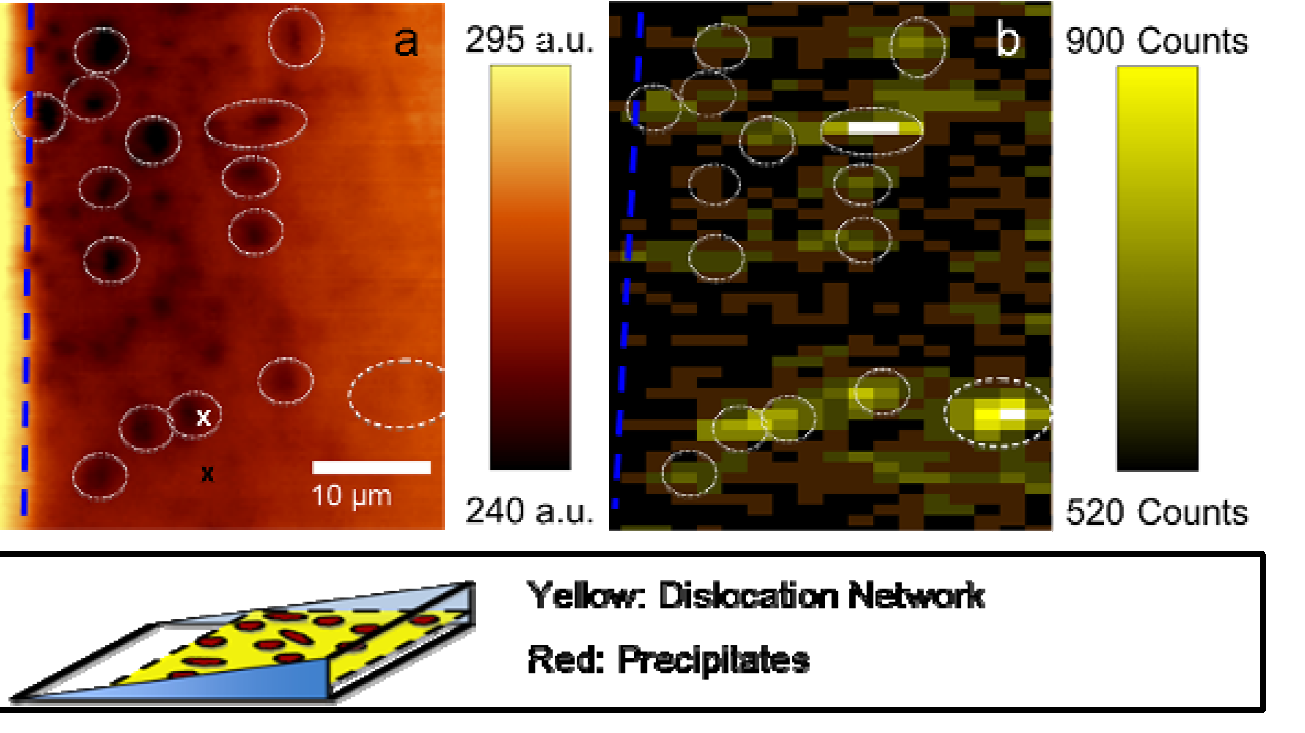
\includegraphics[width=8cm]{gundel_iron_precipitates}%
\caption[Iron precipitates]{Bottom: Scheme of the sample preparation with the polished angle. Top: A Intensity of the BB PL peak at room temperature (a), and of the iron X-ray K$\alpha$ fluorecence (b) from \cite{gundel09}. The dislocation network intersects the surface to the right of the dashed blue line. The white circles show recombination active precipitates.}
\label{fig:gundel_iron_precipitates}%
\end{figure}

Electron hole droplets (EHD), free excitons (FE) and bound excitons (BE) localized on phosphorus atoms has been steadily observed in \cite{drozdov03} with photoluminescence on samples with low-dislocated regions. With increasing dislocation density the FE, BE and EHD bands decrease sharply. This may be due exciton capture by dislocation lines D1,D2 and non-radiative recombination \cite{drozdov03}. EHD photoluminescence intensity is highly dependent on the pumping power \cite{satoshi04}. There is a linear dependence, and pumping with 3~mW or less makes it hardly visible in \cite{satoshi04} with spot size of 1.5~$�$m.

D1 line is shifted towards higher energies under uniaxial elastic deformation of samples with introduced dislocations or after their annealing in oxygen at 750~$^\circ$C \cite{drozdov81}. Room temperature mapping of the 0.77eV band is attributed to oxygen precipitates in thermally treated silicon made by the Czochralski process (Cz-Si) \cite{tajima95}. The increase of this band on the dislocation lines is due to the preferential precipitation of oxygen \cite{tajima95}. Later, \cite{inoue07} state that the deep-level emission from multicrystalline silicon with an intensity maximum at 0.78~eV at room temperature is different from that of the D1 line at low temperature. Furthermore, \cite{inoue07} suggest that the 0.78~eV emission is associated with oxygen precipitation, and that the intra-grain defects are dislocation clusters decorated with oxygen impurities in addition to heavy-metal impurities. \cite{gundel08} state that the origin of trap densities in multicrystalline silicon could be structural crystal defects, which are highly decorated with oxygen precipitates.


%\subsection{Material science}

A commonly used semiconductor for solar cells, is silicon. The supply of silicon is practically endless. 60\% of the Earth's crust is sand, for the major part SiO$_2$. Metallurgical grade silicon (MG-Si) is produced in large amounts to make special steel alloys. Its purity is only 99\% - insufficient for electronic applications \cite{solar_cells}. 

The semiconductor industry purifies this metallurgical-grade silicon until the purity is better than 99.99999~\%. This corresponds to less than 0.1~ppma (part per million atomic), meaning that the total number of foreign atoms must be less than 5$\cdot$10$^{15}$~cm$^{-3}$, due to silicon crystalline atoms density of 5$\cdot$10$^{22}$~cm$^{-3}$ \cite{solar_cells}.

Semiconductor-grade silicon is about ten times more pure than solar-grade silicon. That means that solar-grade silicon can contain up to 1~ppma impurities and still permit reasonably efficient cells. This allows for a lower cost purification process.

\subsubsection{Czochralski method}

The most common crystallization method used for both microelectronoic and photovoltaic industries is the Czochralski method (CZ) ,  shown in figure \ref{fig:czochralski_process} \cite{solar_cells}.

\begin{figure}[H]
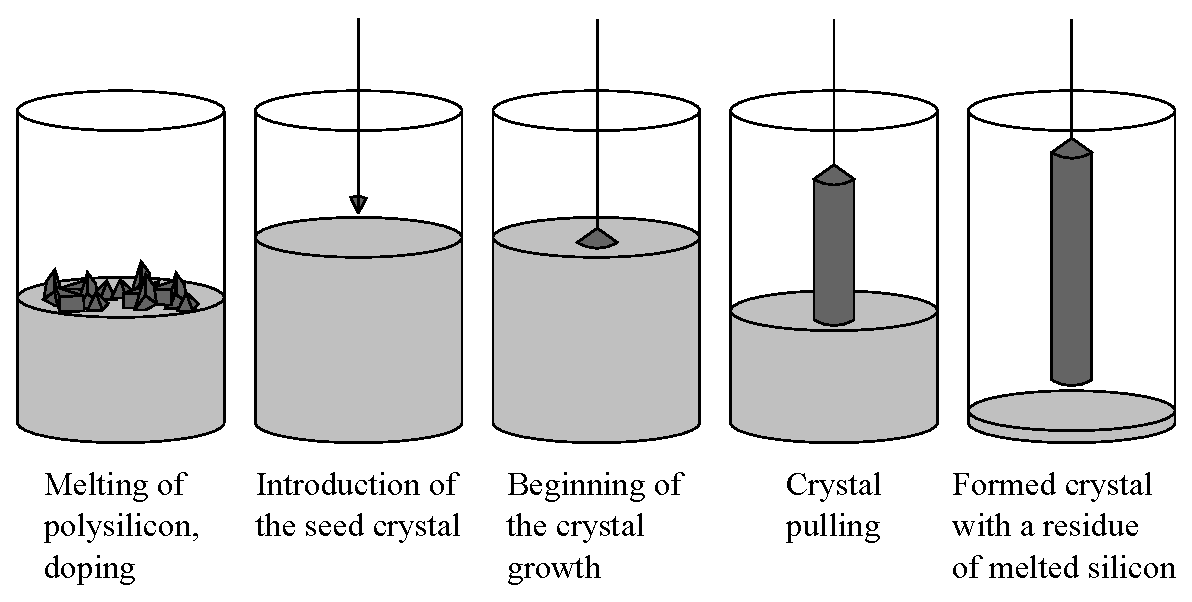
\includegraphics[width=\columnwidth]{Czochralski_Process}%
\caption{Czochralski process}%
\label{fig:czochralski_process}%
\end{figure}

In the CZ crystal growth, silicon chunks are first melted at 1414$^\circ$C in a graphite crucible lined with high purity quartz (SiO$_2$). This known as a feedstock. A small polysilicon crystal is used as a seed to start the crystallization process. The seed is carefully put in contact with the melt and then pulled out very slowly. The temperature is controlled, so that the silicon solidifies at the interface between the seed and the melt and the atoms arrange themselves according to the crystallographic structure of the seed. The crystal grows both vertically and laterally, aided by a rotation movement, yielding a cylindrical ingot of single-crystal silicon. 

The growth rate in the CZ method is about 5~cm/h and the cylindrical ingots are typically 1~m long, 20~cm in diameter and 75~kg in weight \cite{solar_cells}. A disadvantage of the CZ method is that the interaction between the molten silicon and the crucible introduces some contamintants, in particular carbon and oxygen. 

\subsubsection{Float-zone process}

The highest quality silicon crystals are obtained by using the float-zone process. In this method, the starting polysilicon is first given the shape of a cylindrical bar. The bar is then locally melted by a coil using radio frequency induction. By moving the coil, and hence the molten zone, along the bar starting from the seed end, the silicon adopts the crystalline structure. The molten zone is self-supporting and is never in contact with a foreign material, thus avoiding contamination problems. The typical growth rate is 15-30~cm/h, and the typical ingot is 15~cm in diameter and 1~m in length.

\subsubsection{Siemens process}

In the Siemens reactor process, trichlorosilane gas is introduced into a thermal decomposition furnace (reactor) exposing high-purity silicon rods at 1150~$^\circ$C. The trichlorosilane gas decomposes and deposits additional silicon onto the rods, enlarging them:

\begin{equation}
2 \text{HSiCl}_3 \rightarrow 2 \text{HCl} + \text{SiCl}_4
\label{eq:siemens}
\end{equation}

The silicon contained in the gas will deposit on the heated rods, which gradually grow until the desired diameter has been reached. The end product is in the form of rods or chunks of polysilicon. The technology in the Siemens reactor is widely implemented, accounting for a majority of the polysilicon production today, and produce a high purity material \cite{pv_handbook}.


\subsubsection{Multicrystalline silicon}

In order to reduce cost, and increase production rates, the multicrystalline silicon (mc-Si) production method was developed. It is possible to grow silicon ingots by simply melting the starting material, typically silicon scrap, into a crucible, and carefully controlling the cooling rate. Upon cooling, a directional solidification takes place and relatively large crystals grow in a columnar way. A crystalline seed is not used, and the nucleation of the silicon atoms commences in many places simultaneously, leading to a myriad of crystals (or grains) of arbitrary shape and crystallographic orientation. Each grain is several millimeters to centimeters across, and internally it has the same structure as single crystalline silicon. The boundaries between the different grains (grain boundaries), are the most obvious imperfection in the material, but they are not the only ones. Microdefect are also common and contamination from the crucible can happen as well, not to mention the possible impurities present in the starting silicon. This means that the mc-Si typically has lower electronic quality than the material produced by other methods, like the CZ method. Mc-Si typically contains much less oxygen then CZ-Si, due to CZ-Si is more exposed to air during the manufacturing process. The typical crystallization rate is 3.5~kg, and the growth cycle of a complete 16~kg ingot takes 46~h \cite{solar_cells}. 

\subsubsection{Wafers}

The silicon ingots have to be sliced into wafers. Before this they are shaped to meet dimensional specifications. The cylindrical CZ ingots are usually reduced to a quasi-square shape. This implies a loss of about 25~\% of the material, but is necessary if a high packing factor of the cells in the module is required. The large cast silicon parallelepipeds are sawn into smaller bricks. In the case of mc-Si ingots, the shaping is also used to discard the peripheral regions that are usually heavily contaminated by the crucible, which represents approximiately 15~\% of the ingot. In the photovoltaic industry, the wafers are cut by a multi-wire saw machines, that can cut simultaneously whole blocks, thus increasing the throughput dramatically (figure \ref{fig:wire_saw}).

\begin{figure}%
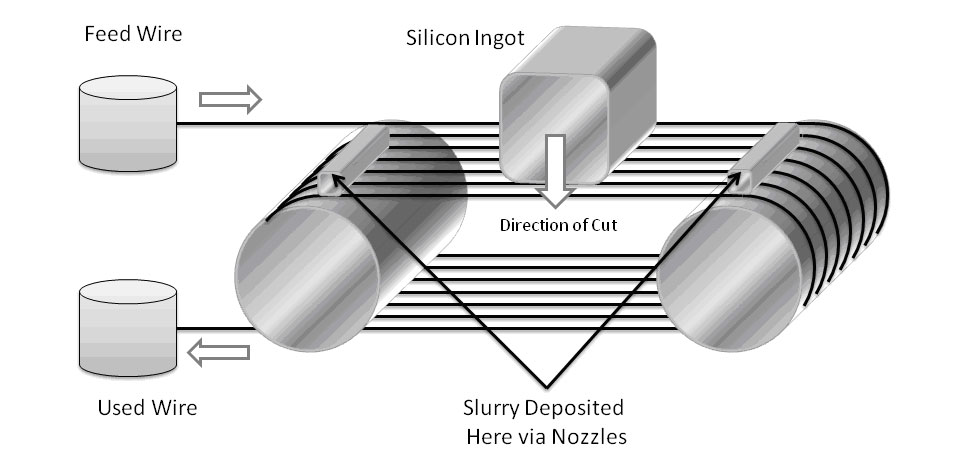
\includegraphics[width=\columnwidth]{wire_saw}%
\caption{Wafer wire saw (figure from \cite{wire_saw})}%
\label{fig:wire_saw}%
\end{figure}

An abrasive slurry helps the steel wires cut through silicon, which is a very hard material. The cutting is very slow, with eight hours being typically needed to cut through a 10x10~cm$^2$ block. Despite this advanced technique, slicing remains as one of the most costly steps of the whole silicon solar cell fabrication. Even if very thin wires are used, approximately 30~\% of the silicon is wasted as saw dust \cite{solar_cells}.


\subsubsection{Doping}

A controlled amount of boron or phosphorus is usually added to the melt (feedstock) to dope the silicon p- or n-type. Rather than the elemental boron or phosphorous, accurately measured amounts of silicon, heavily doped with those elements, are added to the melt. The typical boron concentration used for solar cell applications is 1.5$\cdot$10$^{16}$~cm$^{-3}$, which results in a resistivity of 1~\ohm cm \cite{solar_cells}.


\subsubsection{Defects}

Crystals possess imperfections. They are often referred to as crystalline defects. The presence of most of these crystalline defects is undesirable in silicon wafers. Crystalline defects may be classified into four categories according to their geometry; zero-dimensional or point defects, one-dimensional or line defects, two-dimensional or area defects, and three-dimensional or volume defects

\begin{table}[H]
\begin{tabular}{|c|c|}

\hline
\textbf{Defect type} & \textbf{Examples} \\ \hline

\multirow{4}{*}{Point or zero-dimensional defects} & Vacancy defects \\
 & Interstitial defects \\
 & Frenkel defects \\
 & Extrinsic defects \\ \hline
 
\multirow{2}{*}{Line or one-dimensional defects} & Straight dislocations (edge or screw) \\
 & Dislocation loops \\ \hline
 
\multirow{3}{*}{Area or two-dimensional defects} & Stacking faults \\
 & Twins \\
 & Grain boundaries \\ \hline

\multirow{2}{*}{Volume or three-dimentional defects} & Precipitates \\
 & Voids \\ \hline

\end{tabular}
\caption{Examples of crystalline defects from \cite{siliconfareast}}
\label{tab:crystalline_defects}
\end{table}

Vacancy defects are defects where a silicon atom is missing in the crystal structure. If an atom is located at a non-lattice location within the crystal, it is known as an interstitial defect. If the interstitial defect involves a silicon atom at an interstitial site within a silicon crystal, then it is referred to as a self-interstitial defect. Vacancies and self-interstitial defects are classified as intrinsic point defects \cite{siliconfareast}.
            
A Frenkel defect, is when an atom vacates its position in the crystal lattice to an interstitial position. Extrinsic point defects involve a foreign atom, and are more critical than intrinsic point defects. If this foreign atom replace a silicon atom in the lattice, it becomes a substitutional impurity. This include impurity atoms like the dopants B and P. Other common impurities are oxygen, carbon, and metals \cite{davies88}.


Dislocations, or crystal line defects consists of edge dislocations, screw dislocations or a combination of the two. Edge dislocation can be described as an extra plane of atoms squeezed into a part of the crystal lattice. The location with extra atoms would be under compressive stresses, while the part with correct number of atoms would be under tensile stresses. The line connecting all the atoms at the end of the extra plane is known as the dislocation line.

Screw dislocation is such that a step or ramp is formed by the displacement of atoms in a plane in the crystal. The dislocation line of a screw dislocation is in the axis of the screw.


\begin{figure}[H]
\centering
\subfigure[An edge dislocation]{
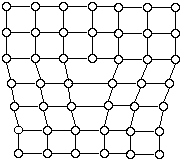
\includegraphics[width=.45\columnwidth]{edge_dislocation}
\label{fig:edge_dislocation}
}
\subfigure[A screw dislocation from \cite{siliconfareast}]{
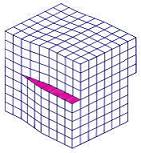
\includegraphics[width=.45\columnwidth]{screw_dislocation}
\label{fig:screw_dislocation}
}
\label{fig:dislocations}
\caption{Dislocations}
\end{figure}

Dislocation loop is a closed curve consisting of an extra plane of atoms lying entirely within the crystal. The line usually form a circular shape, since this shape results in the lowest dislocation energy \cite{siliconfareast}.

Dislocations are not wanted in silicon wafers because impurities are known as recombination centers \cite{tarasov00} and serve as sinks for metallic impurities. Gettering may also occur at dislocations, which can lead to the formation of precipitates.


Stacking faults can be considered as a disturbance in the regularity of the stacking of planes in a crystal lattice. This can occur when a plane is inserted or removed from the lattice. Stacking faults can become electrically active when decorated by impurity atoms. Such stacking faults can lead to device degradation.

A twin is a mirroring of a regular lattice formed during the growth of the silicon ingot. This is usually caused by perturbation. The twin boundary is the mirror plane of the twin formation as seen in figure (\ref{fig:twin_boundary});

\begin{figure}[H]
\centering
\subfigure[Stacking faults from \cite{stacking_faults}]{
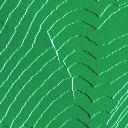
\includegraphics[width=.45\columnwidth]{stacking_fault}
\label{fig:stacking_faults}
}
\subfigure[Twin boundary]{
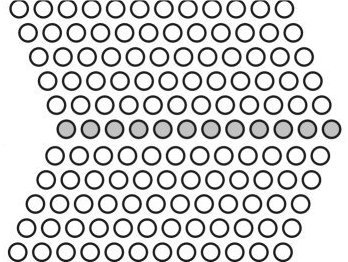
\includegraphics[width=.45\columnwidth]{twin_boundary}
\label{fig:twin_boundary}
}
\label{fig:dislocations_types}
\caption{Area defects}
\end{figure}

Grain boundaries are the boundary in between individual grains where crystal orientation is different from one another. This is common in mc-Si samples due to the production method.
     
Bulk or volume defects include voids and precipitates of extrinsic and intrinsic point defects. Impurities in a crystal which are introduced at a high temperature usually have a higher solubility than for lower temperatures. If the maximum concentration of an impurity allowed by its solubility at high temperature, the crystal become supersaturated with that impurity once it is cooled down. Under such supersaturated conditions, the crystal seeks and achieves equilibrium by precipitating the excess impurity atoms into another plane phase of different composition or structure. Precipitates are undesireable because they can act as sites for generation of dislocations. Precipitates can form in silicon from metallic impurities, oxygen and dopants like boron \cite{siliconfareast}.


